\chapter{PlanetLab Results}

\drop{I}{n} this annex, firstly the bandwidth; then, loss-rate; and finally, latency
plots with the values obtained from the \pl experiment of the selected nodes in Annex~\ref{anex:planetlab-nodes} are depicted.
\clearpage
\section{Bandwidth Plot}
\begin{center}
\begin{figure}[H]
  \centering
  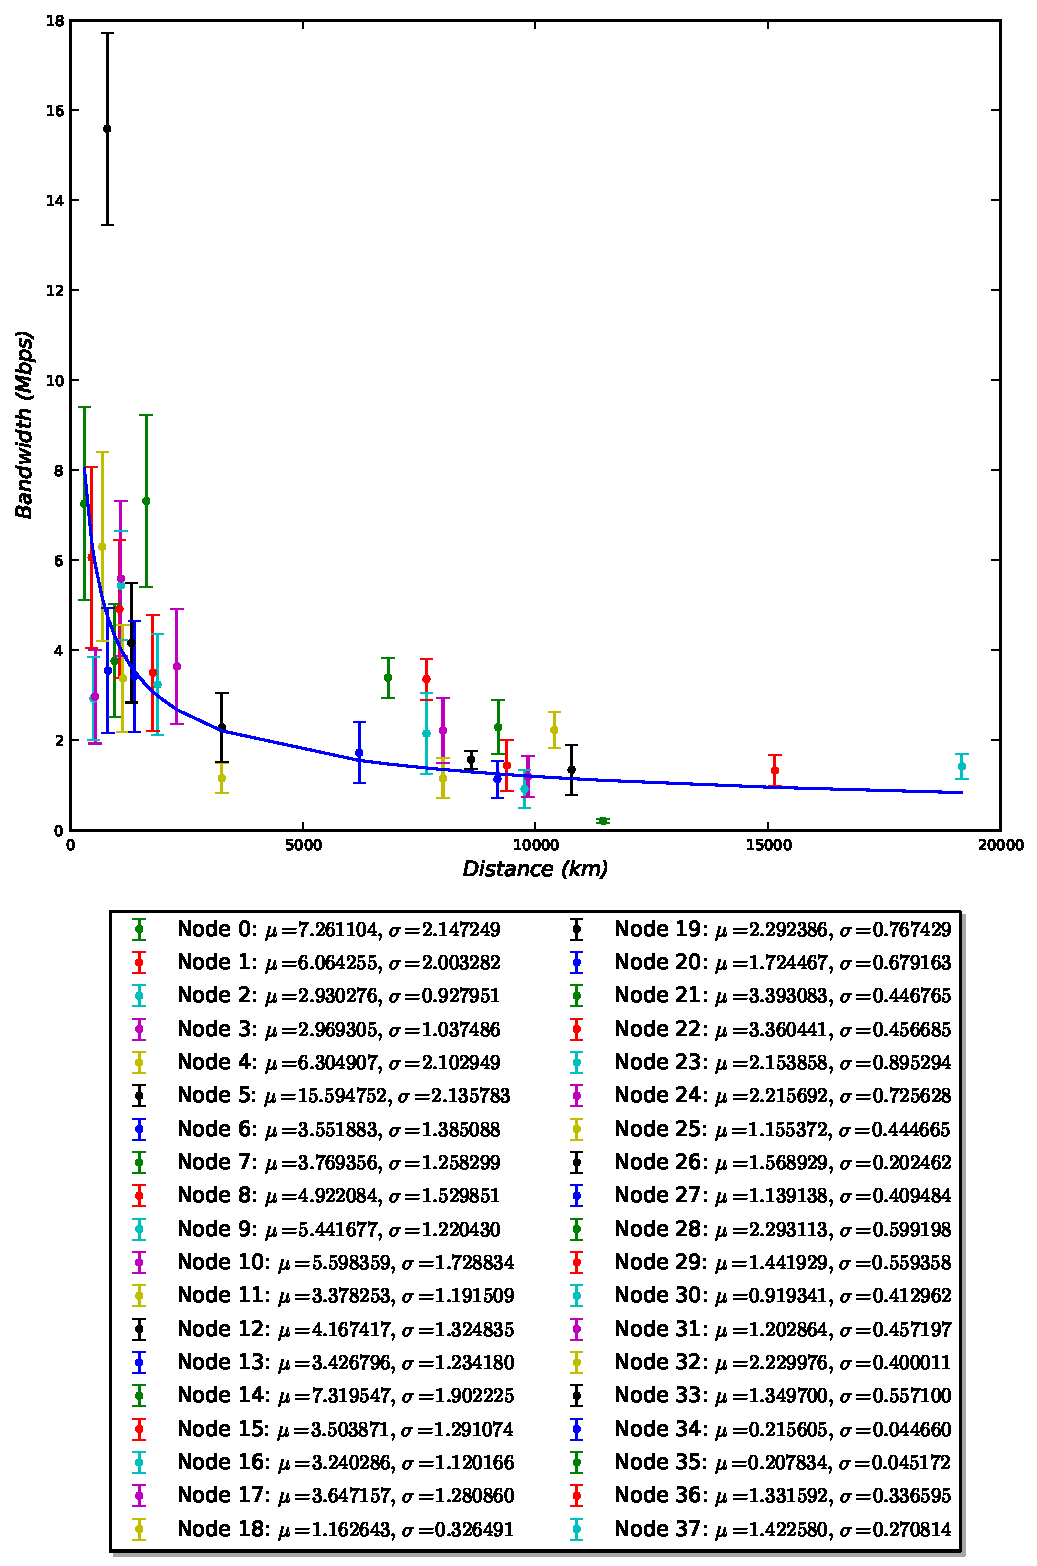
\includegraphics[scale=0.7]{resultsPL/bandwidthall.pdf}\\
  \caption{Bandwidth of all nodes.} \label{fig:bandwidth-plot}
\end{figure}
\end{center}
% \section{Ground Station Bandwidth Histograms}
% \begin{figure}[tb]
%   \centering                        -------pagecommand={\section{Bandwidth Plot}}
%   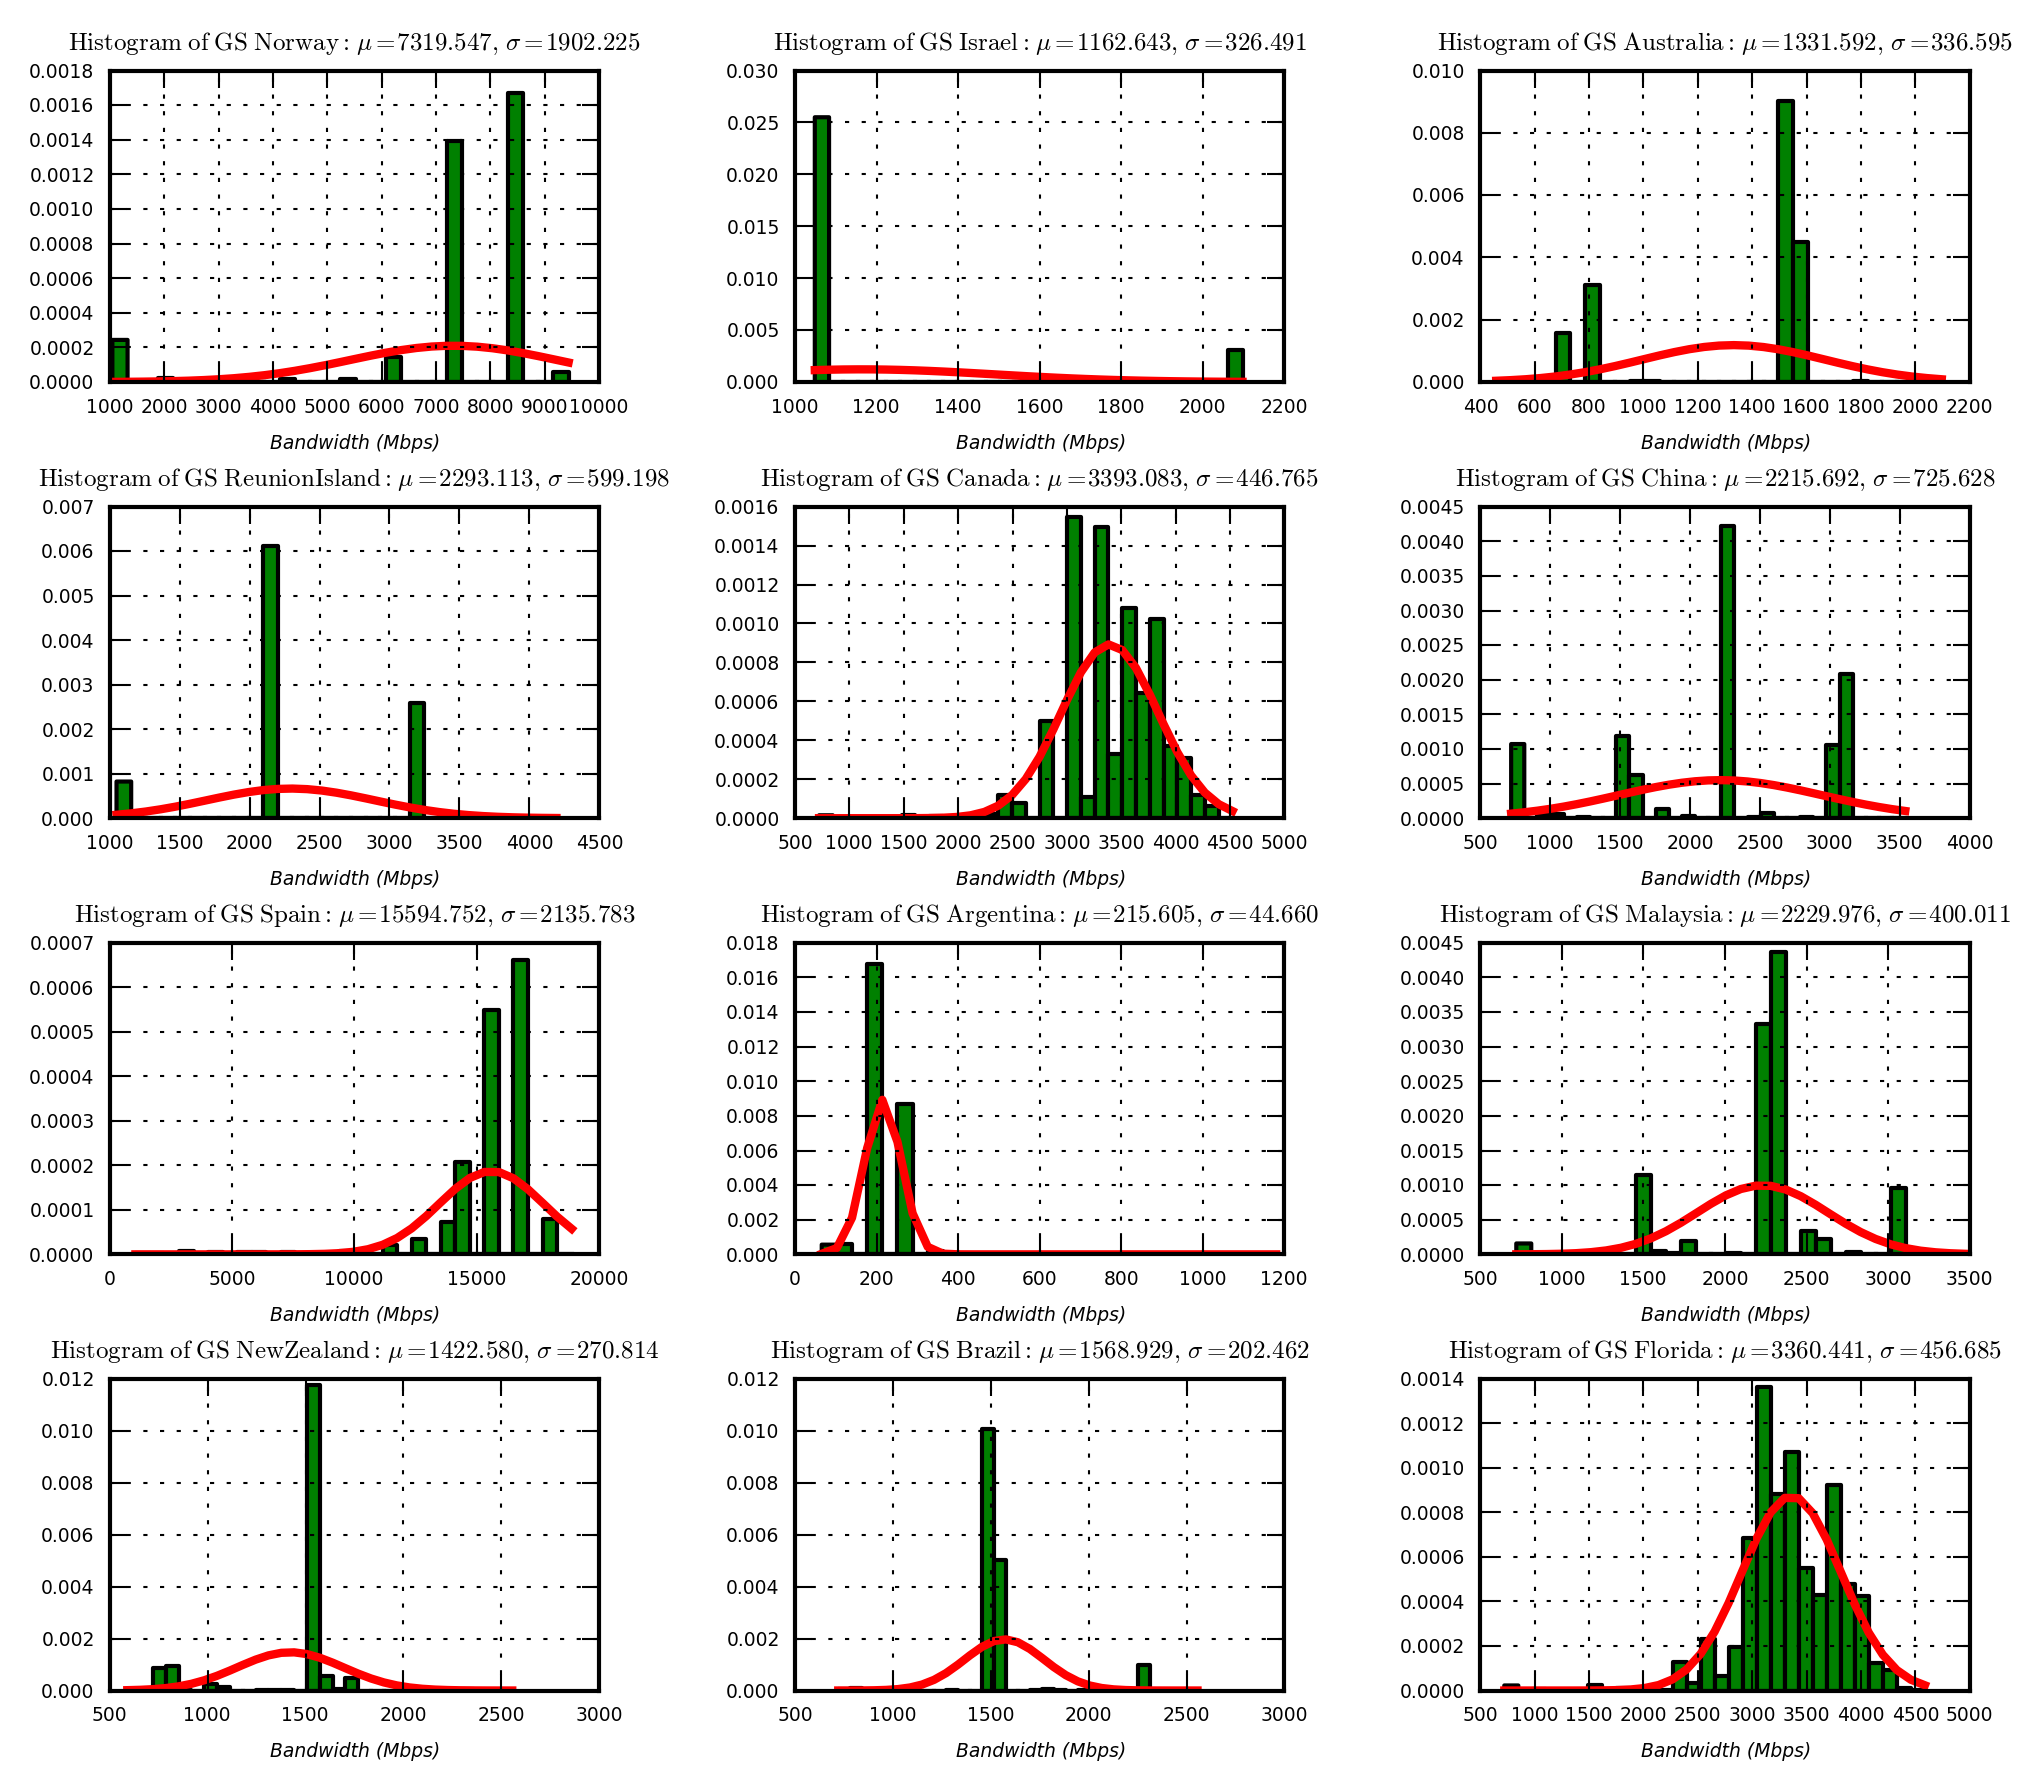
\includegraphics[scale=0.8]{resultsPL/GSGraph.png}\\
%   \caption{Bandwidth of all nodes.} \label{fig:histograms-bandwidth}
% \end{figure}
\clearpage
\section{Delay Plot}
\begin{center}
\begin{figure}[H]
  \centering
  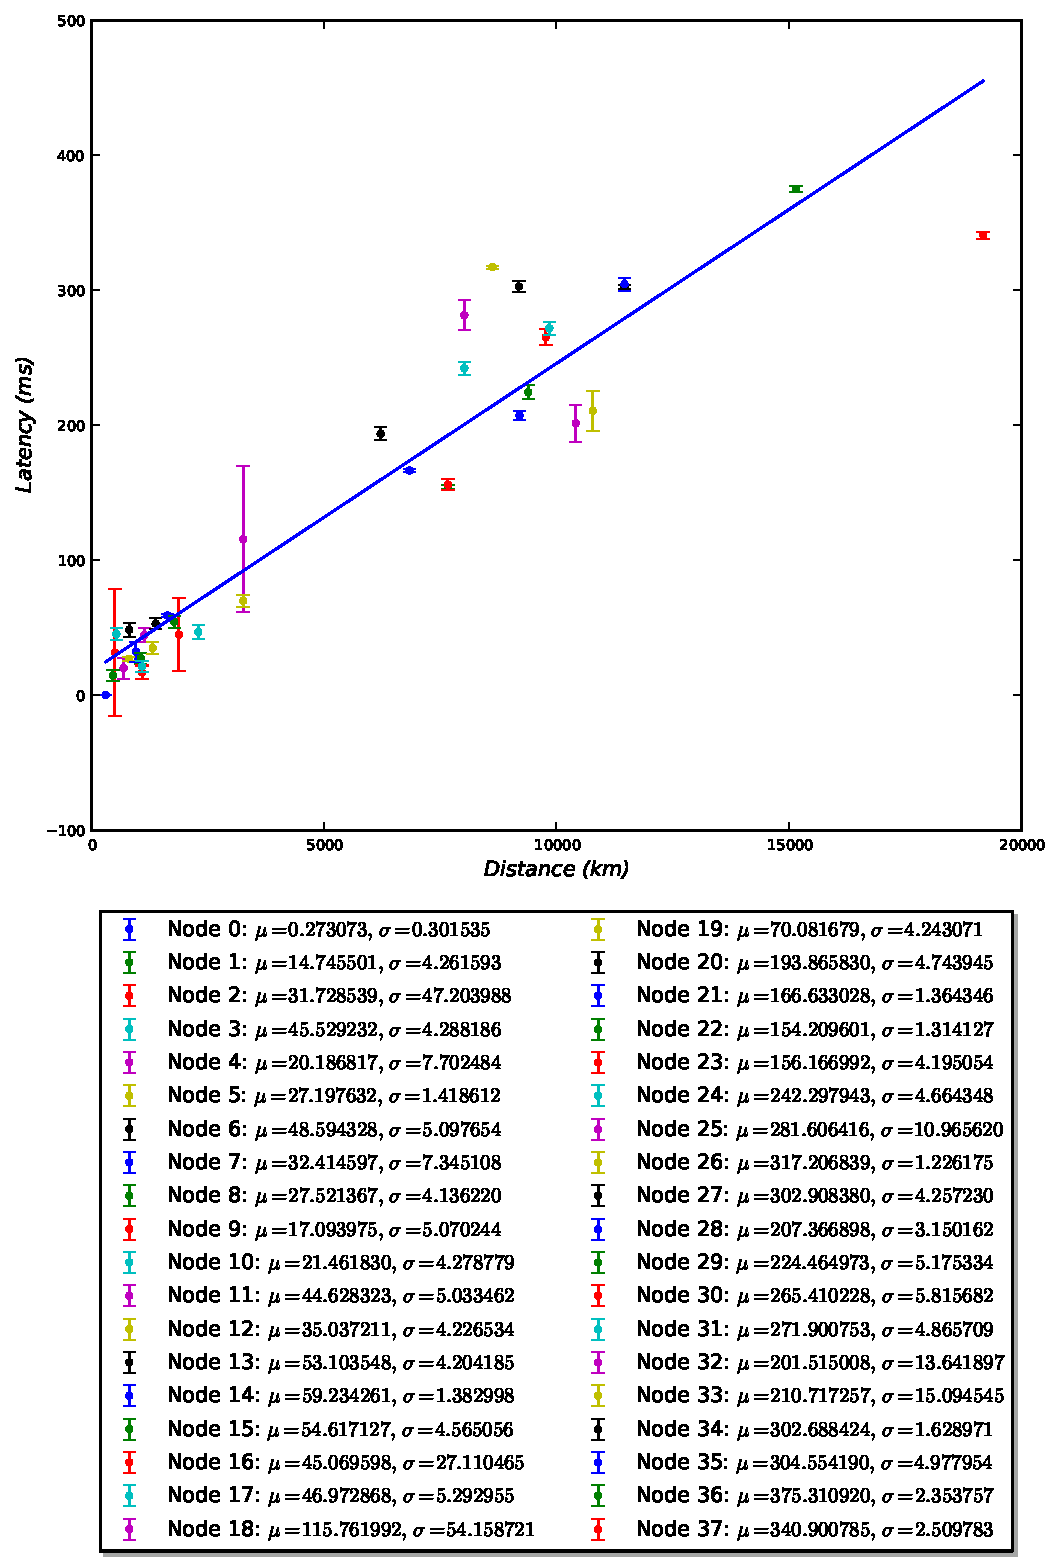
\includegraphics[scale=0.7]{resultsPL/DelayNodes.pdf}\\
  \caption{Bandwidth of all nodes.} \label{fig:delay-plot}
\end{figure}
\end{center}
\clearpage
\section{Loss-Rate Plot}
\begin{center}
\begin{figure}[H]
  \centering
  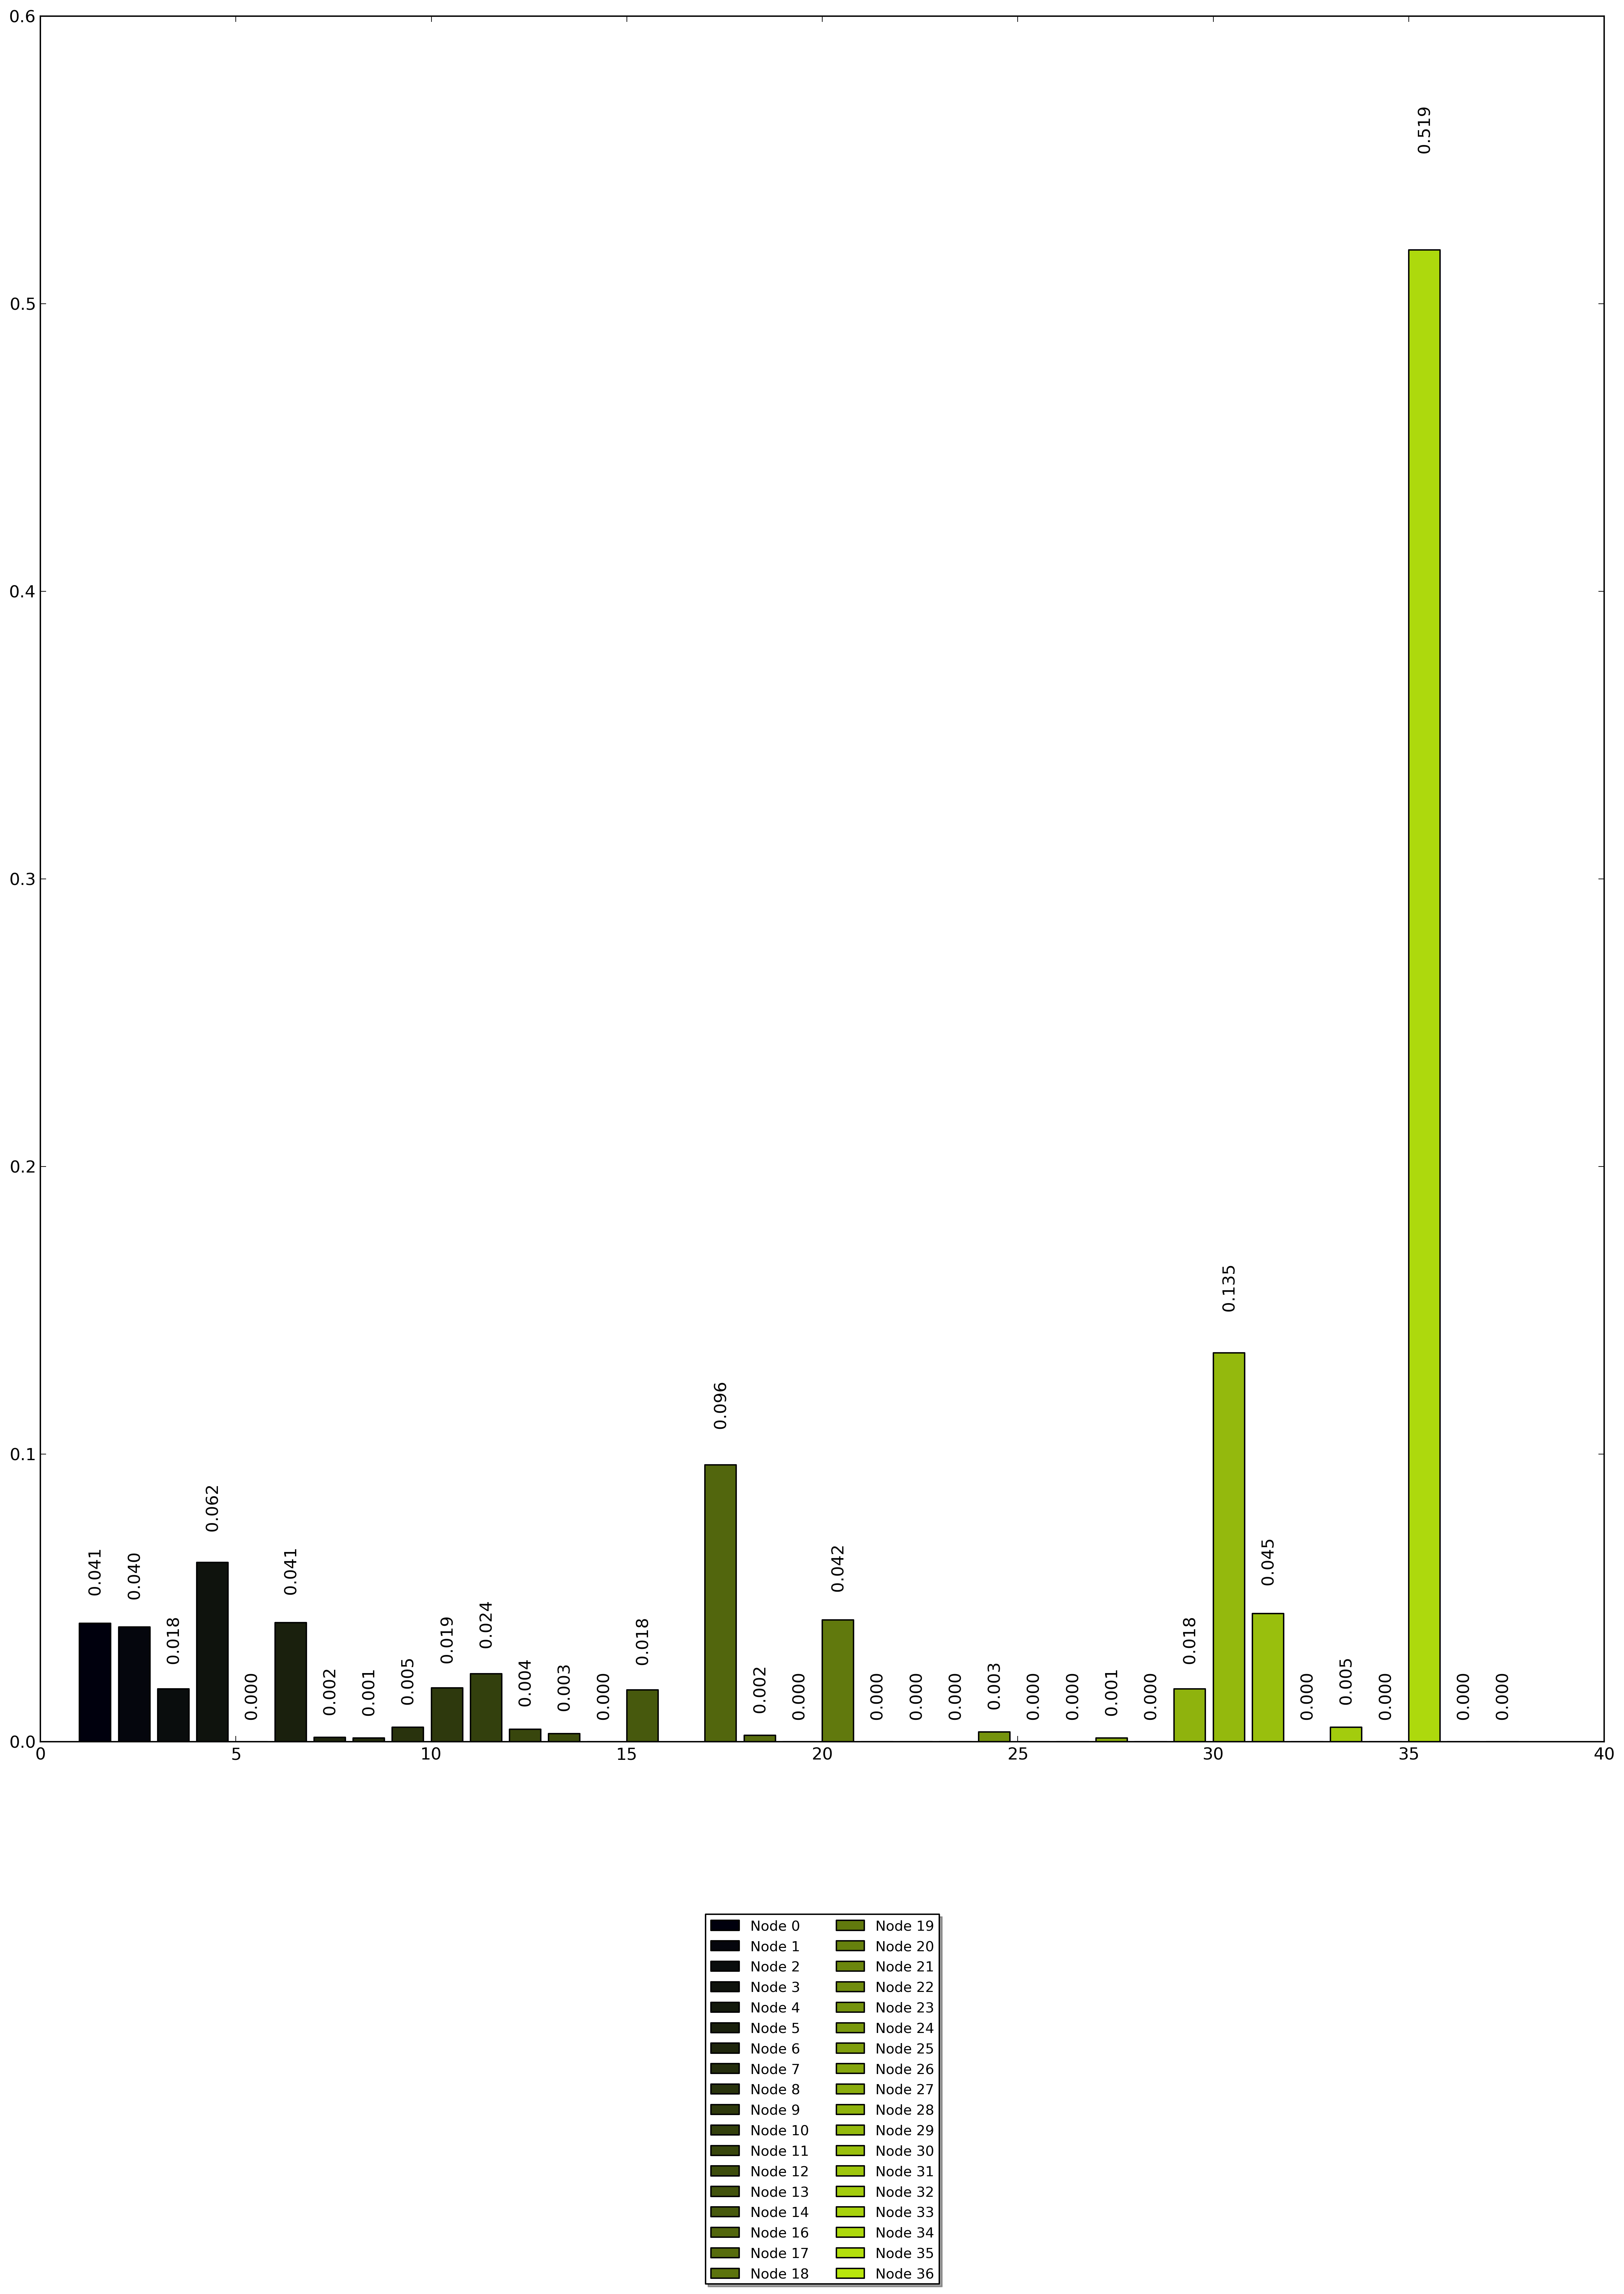
\includegraphics[scale=0.6]{resultsPL/Loss-rateALL.png}\\
  \caption{Bandwidth of all nodes.} \label{fig:loss-rate-plot}
\end{figure}
\end{center}
\clearpage
\section{Summary Table}
The following table represents every selected nodes and their loss-rate,
bandwidth and latency measured values. The meaning of columns are the following:
$CN$ means Central Node; $BW$ means Bandwidth; $\mu$ means mean; $\sigma$ means
standard deviation and $\#$ means Number.


\begin{landscape}
% \begin{table}[hp]
%   \centering
%   {\small
%   

\begin{center}
{\small
\begin{longtable}{c c c c c c c c c}

\tabheadformat
\tabhead{Country} & \tabhead{Selected Node} & \tabhead{$\#$} & \tabhead{Layer}
&\tabhead{BW $\mu$} & \tabhead{BW $\sigma$ }
&\tabhead{Latency $\mu$}
&\tabhead{Latency $\sigma$ } &\tabhead{Loss Rate}\\
\tabheadformat
               &                         &               &                &
\tabhead{[Mbps]}   &\tabhead{[Mbps]}          &        \tabhead{[ms]}          &
\tabhead{[ms]}                &    \tabhead{$\%$}\\\hline
\endhead
        France & ple6.ipv6.lip6.fr                      & CN &1.2 &N/A&N/A&N/A&N/A&N/A\\\hline
        France & inriarennes2.irisa.fr                  & 0   &  2 &7.261104&2.147249&0.273073&0.301535&0.041\\\hline
        Switzerland & planetlab2.unineuchatel.ch        & 1   &  2 &6.064255&2.003282&14.745501&4.261593&0.040\\\hline
        Belgium & rochefort.infonet.fundp.ac.be         & 2   &  2 &2.930276&0.927951&31.728539&47.203988&0.018\\\hline
        Spain & dplanet2.uoc.edu                        & 3   &  2 &2.969305&1.037486&45.529232&4.288186&0.148\\\hline
        Netherlands & planetlab1.cs.vu.nl               & 4   &  2 &6.304907&2.102949&20.186817&7.702484&0.062\\\hline
        Spain & Planetlab2.dit.upm.es                   & 5   &  1 &15.594752&2.135783&27.197632&1.418612&0.005\\\hline
        Germany & planetlab02.tkn.tu-berlin.de          & 6   &  2 &3.551883&1.385088&48.594328&5.097654&0.041\\\hline
        Italy & planet-lab-node1.netgroup.uniroma2.it   & 7   &  2 &3.769356&1.258299&32.414597&7.345108&0.002\\\hline
        Czech Republic & planetlab1.cesnet.cz           & 8   &  2 &4.922084&1.529851&27.521367&4.136220&0.001\\\hline
        United Kingdom & planetlab-2.imperial.ac.uk     & 9   &  2 &5.441677&1.220430&17.093975&5.070244&0.005\\\hline
        Ireland & planetlab-node-01.ucd.ie              & 10  &  2 &5.598359&1.728834&21.461830&4.278779&0.019\\\hline
        Portugal & planet1.servers.ua.pt                & 11  &  2 &3.378253&1.191509&44.628323&5.033462&0.024\\\hline
        Hungary & planet2.elte.hu                       & 12  &  2 &4.167417&1.324835&35.037211&4.226534&0.004\\\hline
        Poland & ple2.dmcs.p.lodz.pl                    & 13  &  2 &3.426796&1.234180&53.103548&4.204185&0.003\\\hline
        Norway & planetlab1.cs.uit.no                   & 14  &1.2 &7.319547&1.902225&59.234261&1.382998&0.006\\\hline
        Greece & planetlab1.ionio.gr                    & 15  &  2 &3.503871&1.291074&54.617127&4.565056&15.68\\\hline
        Sweden & planetlab2.s3.kth.se                   & 16  &  2 &3.240286&1.120166&45.069598&27.110465&0.096\\\hline
        Finland & planetlab-1.research.netlab.hut.fi    & 17  &  2 &1.120166&1.280860&46.972868&5.292955&0.002\\\hline
        Israel & planetlab2.tau.ac.il                   & 18  &  2 &1.162643&0.326491&115.761992&54.158721&0.042\\\hline
        Israel & planet1.cs.huji.ac.il                  & 19  &  1 &2.292386&0.767429&70.081679&4.243071&0.001\\\hline
        Russian Federation & plab1.cs.msu.ru            & 20  &  2 &1.724467&0.679163&193.865830&4.743945&0.000\\\hline
        Canada & planetlab-2.usask.ca                   & 21  &1.2 &3.393083&0.446765&166.633028&1.364346&0.008\\\hline
        USA & Planetlab1.eecs.ucf.edu                   & 22  &  1 &3.360441&0.456685&154.209601&1.314127&0.010\\\hline
        United States & planetlab-04.cs.princeton.edu   & 23  &  2 &2.153858&0.895294&156.166992&4.195054&0.003\\\hline
        China & planetlab1.buaa.edu.cn                  & 24  &  1 &2.215692&0.725628&242.297943&4.664348&0.024\\\hline
        China & planetlab1.cqupt.edu.cn                 & 25  &  2 &1.155372&0.444665&281.606416&10.965620&0.048\\\hline
        Brazil & planetlab1.pop-pa.rnp.br               & 26  &1.2 &1.568929&0.202462&317.206839&1.226175&0.076\\\hline
        Korea, Republic of & netapp7.cs.kookmin.ac.kr   & 27  &  2 &1.139138&0.409484&302.908380&4.257230&0.001\\\hline
        Reunion Island, France & lim-planetlab-1.univ-reunion.fr & 28 & 1  &2.293113&0.599198&207.366898&3.150162&0.010\\\hline
        Thailand & ple2.ait.ac.th                       & 29  &  2 &1.441929&0.559358&224.464973&5.175334&0.018\\\hline
        Hong Kong & planetlab1.ie.cuhk.edu.hk           & 30  &  2 &0.919341&0.412962&265.410228&5.815682&0.135\\\hline
        Japan & planet1.pnl.nitech.ac.jp                & 31  &  2 &1.202864&0.457197&271.900753&4.865709&0.045\\\hline
        Malaysia & planetlab1.comp.nus.edu.sg           & 32  &  1 &2.229976&0.400011&201.515008&13.641897&0.063\\\hline
        Singapore & planetlab1.comp.nus.edu.sg          & 33  &  2 &1.349700&0.557100&210.717257&15.094545&0.005\\\hline
        Argentina & planet-lab2.itba.edu.ar             & 34  &  1 &0.215605&0.044660&302.688424&1.628971&0.240\\\hline
        Argentina  & planet-lab2.uba.ar                 & 35  &  2 &0.207834&0.045172&304.554190&4.977954&0.519\\\hline
        Australia & pl1.eng.monash.edu.au               & 36  &1.2 &1.331592&0.336595&375.310920&2.353757&0.004\\\hline
        New Zealand & planetlab1.cs.otago.ac.nz         & 37  &1.2 &1.422580&0.270814&340.900785&2.509783&0.204\\\hline
\caption{Obtained values of PlanetLab Experiment}
\label{anex:nodes-pl-results}
\end{longtable}
}
\end{center}

%   }
%   \caption{Impairments in PlanetLab nodes}
%   \label{table:ple-results-impairments}
% \end{table}
 

\begin{center}
{\small
\begin{longtable}{c c c c c c c c c}

\tabheadformat
\tabhead{Country} & \tabhead{Selected Node} & \tabhead{$\#$} & \tabhead{Layer}
&\tabhead{BW $\mu$} & \tabhead{BW $\sigma$ }
&\tabhead{Latency $\mu$}
&\tabhead{Latency $\sigma$ } &\tabhead{Loss Rate}\\
\tabheadformat
               &                         &               &                &
\tabhead{[Mbps]}   &\tabhead{[Mbps]}          &        \tabhead{[ms]}          &
\tabhead{[ms]}                &    \tabhead{$\%$}\\\hline
\endhead
        France & ple6.ipv6.lip6.fr                      & CN &1.2 &N/A&N/A&N/A&N/A&N/A\\\hline
        France & inriarennes2.irisa.fr                  & 0   &  2 &7.261104&2.147249&0.273073&0.301535&0.041\\\hline
        Switzerland & planetlab2.unineuchatel.ch        & 1   &  2 &6.064255&2.003282&14.745501&4.261593&0.040\\\hline
        Belgium & rochefort.infonet.fundp.ac.be         & 2   &  2 &2.930276&0.927951&31.728539&47.203988&0.018\\\hline
        Spain & dplanet2.uoc.edu                        & 3   &  2 &2.969305&1.037486&45.529232&4.288186&0.148\\\hline
        Netherlands & planetlab1.cs.vu.nl               & 4   &  2 &6.304907&2.102949&20.186817&7.702484&0.062\\\hline
        Spain & Planetlab2.dit.upm.es                   & 5   &  1 &15.594752&2.135783&27.197632&1.418612&0.005\\\hline
        Germany & planetlab02.tkn.tu-berlin.de          & 6   &  2 &3.551883&1.385088&48.594328&5.097654&0.041\\\hline
        Italy & planet-lab-node1.netgroup.uniroma2.it   & 7   &  2 &3.769356&1.258299&32.414597&7.345108&0.002\\\hline
        Czech Republic & planetlab1.cesnet.cz           & 8   &  2 &4.922084&1.529851&27.521367&4.136220&0.001\\\hline
        United Kingdom & planetlab-2.imperial.ac.uk     & 9   &  2 &5.441677&1.220430&17.093975&5.070244&0.005\\\hline
        Ireland & planetlab-node-01.ucd.ie              & 10  &  2 &5.598359&1.728834&21.461830&4.278779&0.019\\\hline
        Portugal & planet1.servers.ua.pt                & 11  &  2 &3.378253&1.191509&44.628323&5.033462&0.024\\\hline
        Hungary & planet2.elte.hu                       & 12  &  2 &4.167417&1.324835&35.037211&4.226534&0.004\\\hline
        Poland & ple2.dmcs.p.lodz.pl                    & 13  &  2 &3.426796&1.234180&53.103548&4.204185&0.003\\\hline
        Norway & planetlab1.cs.uit.no                   & 14  &1.2 &7.319547&1.902225&59.234261&1.382998&0.006\\\hline
        Greece & planetlab1.ionio.gr                    & 15  &  2 &3.503871&1.291074&54.617127&4.565056&15.68\\\hline
        Sweden & planetlab2.s3.kth.se                   & 16  &  2 &3.240286&1.120166&45.069598&27.110465&0.096\\\hline
        Finland & planetlab-1.research.netlab.hut.fi    & 17  &  2 &1.120166&1.280860&46.972868&5.292955&0.002\\\hline
        Israel & planetlab2.tau.ac.il                   & 18  &  2 &1.162643&0.326491&115.761992&54.158721&0.042\\\hline
        Israel & planet1.cs.huji.ac.il                  & 19  &  1 &2.292386&0.767429&70.081679&4.243071&0.001\\\hline
        Russian Federation & plab1.cs.msu.ru            & 20  &  2 &1.724467&0.679163&193.865830&4.743945&0.000\\\hline
        Canada & planetlab-2.usask.ca                   & 21  &1.2 &3.393083&0.446765&166.633028&1.364346&0.008\\\hline
        USA & Planetlab1.eecs.ucf.edu                   & 22  &  1 &3.360441&0.456685&154.209601&1.314127&0.010\\\hline
        United States & planetlab-04.cs.princeton.edu   & 23  &  2 &2.153858&0.895294&156.166992&4.195054&0.003\\\hline
        China & planetlab1.buaa.edu.cn                  & 24  &  1 &2.215692&0.725628&242.297943&4.664348&0.024\\\hline
        China & planetlab1.cqupt.edu.cn                 & 25  &  2 &1.155372&0.444665&281.606416&10.965620&0.048\\\hline
        Brazil & planetlab1.pop-pa.rnp.br               & 26  &1.2 &1.568929&0.202462&317.206839&1.226175&0.076\\\hline
        Korea, Republic of & netapp7.cs.kookmin.ac.kr   & 27  &  2 &1.139138&0.409484&302.908380&4.257230&0.001\\\hline
        Reunion Island, France & lim-planetlab-1.univ-reunion.fr & 28 & 1  &2.293113&0.599198&207.366898&3.150162&0.010\\\hline
        Thailand & ple2.ait.ac.th                       & 29  &  2 &1.441929&0.559358&224.464973&5.175334&0.018\\\hline
        Hong Kong & planetlab1.ie.cuhk.edu.hk           & 30  &  2 &0.919341&0.412962&265.410228&5.815682&0.135\\\hline
        Japan & planet1.pnl.nitech.ac.jp                & 31  &  2 &1.202864&0.457197&271.900753&4.865709&0.045\\\hline
        Malaysia & planetlab1.comp.nus.edu.sg           & 32  &  1 &2.229976&0.400011&201.515008&13.641897&0.063\\\hline
        Singapore & planetlab1.comp.nus.edu.sg          & 33  &  2 &1.349700&0.557100&210.717257&15.094545&0.005\\\hline
        Argentina & planet-lab2.itba.edu.ar             & 34  &  1 &0.215605&0.044660&302.688424&1.628971&0.240\\\hline
        Argentina  & planet-lab2.uba.ar                 & 35  &  2 &0.207834&0.045172&304.554190&4.977954&0.519\\\hline
        Australia & pl1.eng.monash.edu.au               & 36  &1.2 &1.331592&0.336595&375.310920&2.353757&0.004\\\hline
        New Zealand & planetlab1.cs.otago.ac.nz         & 37  &1.2 &1.422580&0.270814&340.900785&2.509783&0.204\\\hline
\caption{Obtained values of PlanetLab Experiment}
\label{anex:nodes-pl-results}
\end{longtable}
}
\end{center}

\end{landscape}
